\begin{enumerate}
	\item Genere dos vectores aleatorios $R$, $S$ de tamaño $1x11$, tal que cada uno de sus elementos
		sean números primos pertenecientes al intervalo $[1,\ldots,211]$.

	\textbf{R:}\\

R = [37 13 163 131 137 199 139 173  79  47 139] \\
S = [139 173  43 103 173  47  89 109  37 181  83] \\
 
	\item Calcule el valor de $RxS$, $R.S$, $R*S'$, ¿Cual es la diferencia entre cada una de estas
operaciones?, ¿existe alguna información útil que podamos saber de estas?.

	\textbf{R:}\\

	El producto cruz normalmente está definido sólo para $R^3$,
	de todas formas es posible calcularlo para un espacio de $n$ dimensiones,
	pero es necesario contar con al menos $n-1$ vectores,
	finalmente no se puede realizar, ya que falta información\\

	$R$.$S$ = 115143 \\
	$R$*$S$' = 115143 \\

	Dado que los componentes de los vectores, el operador conjugación no realiza grandes cambios en los componentes en si de $S$, 
	por lo que se obtiene una operación equivalente.

	\item Calcule un Vector normal para el vector $R$ y para el vector $S$.

	\textbf{R:}\\

	Para calcular un vector normal N a $R$ y $S$, debe cumplirse que: \\

	$R$.$N_1$ = 0 \\
	$S$.$N_2$ = 0 \\

	Debido a que poseemos 11 incógnitas y 1 ecuación en cada caso, asumimos cualquier valor para los primeros 
	10 componentes del vector N, para luego despejar el componente 11: \\

	$N_1$ = [1.0 1.0 1.0 1.0 1.0 1.0 1.0 1.0 1.0 1.0 -8.0432] \\
	$N_2$ = [1.0  1.0  1.0  1.0  1.0  1.0  1.0  1.0  1.0  1.0 -13.1807] \\
	\newpage
	\item Calcule el ángulo entre los vectores generados.

	\textbf{R:}\\

	$R.S = |R||S| Cos(\phi)$
	$\Leftrightarrow \phi = Cos^{-1}\frac{R.S}{|R||S|} = 46.463^{\circ}$\\

	\item Genere dos vectores con las primeras 3 columnas de $R$ y $S$, grafique los dos nuevos vectores,
		identifique de forma clara cada uno de los vectores.

	\textbf{R:}\\

	r = [37  13 163] \\
	s = [139 173  43] \\

	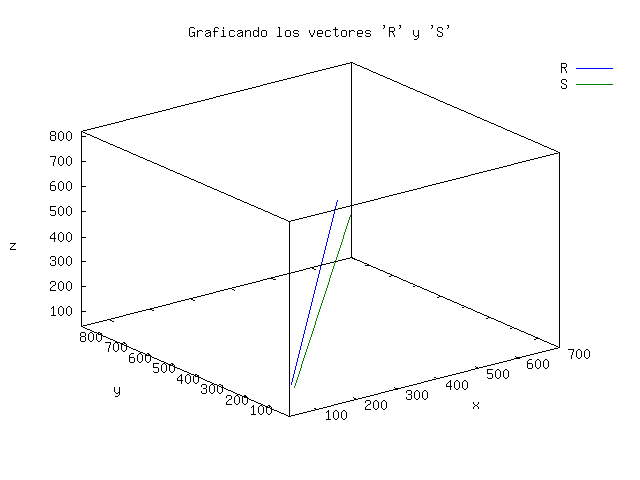
\includegraphics[scale=0.6]{imagenes/vectores.png}

\end{enumerate}

